\documentclass{article}


\usepackage{arxiv}

\usepackage[utf8]{inputenc} % allow utf-8 input
\usepackage[T1]{fontenc}    % use 8-bit T1 fonts
\usepackage{hyperref}       % hyperlinks
\usepackage{url}            % simple URL typesetting
\usepackage{booktabs}       % professional-quality tables
\usepackage{amsfonts}       % blackboard math symbols
\usepackage{microtype}      % microtypography
\usepackage{graphicx}
\graphicspath{ {./images/} }

\title{Real-Time Depth Sensing by Combining Computer Vision and LIDAR Point-Cloud Data}

\date{May 22, 2018}

\author{
  Kin-Ho Lam\\
  College of Engineering\\
  Oregon State University \\
  \texttt{kinholam5@gmail.com}\\
}

\begin{document}
\maketitle

\begin{abstract}
  Modern self-driving car systems face a massive challenge: creating a holistic system capable of accurately identifying obstacles and quickly calculating their distances in real time.
  Such challenges are nontrivial because one must consider multiple conflicting sensory interferences.
  Ambient light from the Sun, reflective surfaces, darkness, fog, and other sensory obsurements pose significant challenges to guaranteeing an autonomous driving system's safety.
  Infrared depth-sensors such as devices used in the Microsoft Kinect promise high depth and object recognition accuracy but fail to work reliably in direct sunlight.
  Computer vision machine learning models are capable of object recognition and depth perception, but only to a degree of certainty.
  LIDAR (Light Imaging Detection and Ranging) sensors are capable of high-accuracy depth sensing, but are affected by fog and are only able to collect point cloud data in a single plane.
  This project seeks to be a proof of concept system that achieves reliable real-time object detection and depth sensing by combining a computer vision model and live LIDAR point-cloud data.
\end{abstract}


% keywords can be removed
\keywords{Depth sensor \and LIDAR \and Computer Vision}

\section{Introduction}
    As the prevalence of automation in our daily lives increases, such as autonomous cars or robots, a cheap and scalable depth sensing system that is resistant to common interferences is necessary.
		The goal of this project is to create a reliable depth sensing system using computer vision and LIDAR.
		Such a system that combines these two technologies will be more reliable than infrared depth sensing because cameras and LIDAR devices are less prone to interference from ambient light or anomalies.

\section{Design}
\label{sec:Design}
    The Logitech Brio webcam provides a high-resolution, two-dimensional image but lacks depth perception.
		The LIDAR provides accurate depth measurement in a horizontal dimension but lacks vertical perspective.
		This project proposes bridging the utility of both devices by securing them in stationary positions, then using software to combine their outputs.
		This involves using the M16 LIDAR to get depth sensing information and using computer vision to recognize objects.
		The result is a scalable and reliable depth sensor that will not be affected by natural light, and can be further improved by training a better computer vision model or adding more sensors.
		This project hopes to achieve a proof of concept design to be showcased in a live demo at Oregon State University's 2018 Undergraduate engineering expo.			
		This live demo shall consist of the full system pointed at the project booth's audience. 

		Figure \ref{fig:fig1}  illustrates different dimensions measured by the M16 LIDAR and Brio Webcam.
		The red cube represents the Logitech Brio webcam and M16 LIDAR secured in stationary positions.
		The flat purple triangle represents the M16 LIDAR's horizontal range detection.
		The transparent green rectangle in front of the person represents the computer vision model recognizing that there is a person in-front of the sensor.
    The transparent teal pyramid represents the Brio webcam's field-of-view.

    \begin{figure}
      \centering
      \fbox{	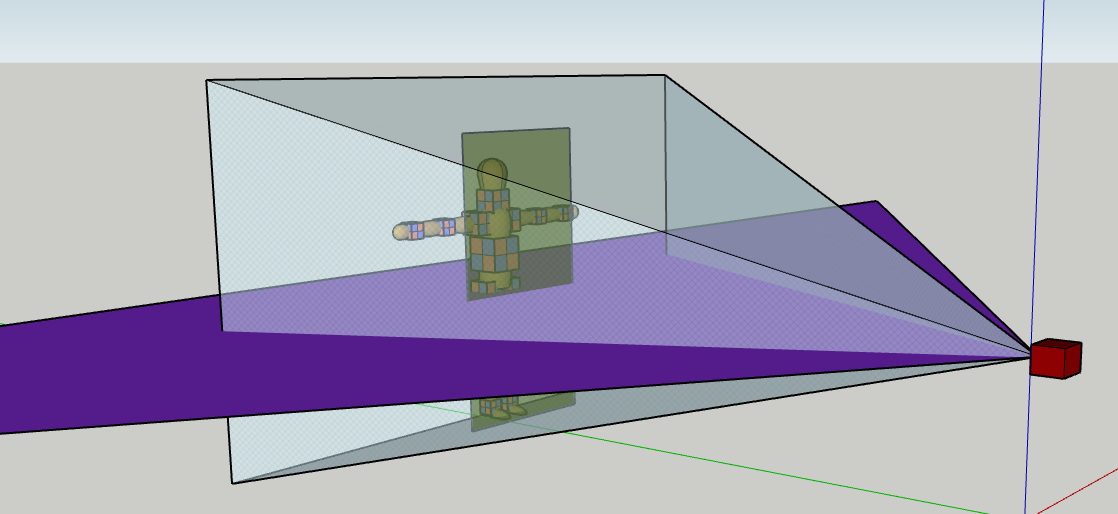
\includegraphics[scale=0.5]{different_dimensions.PNG} }
      \caption{Visualizing different dimensions measured by the LIDAR and Brio Webcam.}
      \label{fig:fig1}
    \end{figure}



\subsection{Headings: second level}
Donec id tempus est. Phasellus feugiat dapibus ultricies. Morbi nec dui nisl. Phasellus cursus justo quis ex rhoncus, congue laoreet turpis tempor. Praesent pharetra tempus dolor, vel convallis felis venenatis vitae. Suspendisse vel dictum magna. Pellentesque consequat cursus euismod. Vestibulum nec luctus sapien. Donec malesuada metus ut velit accumsan fermentum. Nam nec lobortis purus, euismod rhoncus sem. Phasellus vestibulum dapibus condimentum. Nunc mattis erat eu ligula mollis scelerisque. 

\begin{equation} \label{eq1}
  \theta \leq  55:
  X = \frac{video width}{2} * sin(\theta) + \frac{video width}{2}\\
\end{equation}
\\
\begin{equation} \label{eq2}
  \theta \geq 305:
  X = \frac{video width}{2} * sin(360 - \theta)\\
\end{equation}
  

\subsubsection{Headings: third level}
Morbi pharetra aliquam diam vel tincidunt. Nunc eget dui dictum, scelerisque dolor suscipit, finibus orci. In hac habitasse platea dictumst. Sed consequat facilisis nibh, quis porta neque iaculis a. Nullam libero ipsum, facilisis at arcu vitae, accumsan placerat dolor. Duis non viverra urna, in consequat nisl. Aenean ut purus quis nisl efficitur mattis. Nulla facilisi. Etiam nec gravida erat. Sed tempus, felis in tincidunt eleifend, massa leo facilisis odio, nec ornare sapien diam vitae massa. Maecenas porttitor auctor felis, ut venenatis dui venenatis et. Mauris tincidunt, erat quis euismod tempor, velit arcu pharetra orci, eu eleifend nulla risus ac neque. Cras dapibus libero volutpat diam sollicitudin eleifend. 


\paragraph{Paragraph}
Sed faucibus diam eget augue consectetur, fermentum tempor urna efficitur. Donec vitae tempus nulla, ut rhoncus purus. Maecenas fermentum vehicula turpis ac luctus. Suspendisse potenti. Fusce est sapien, rhoncus et fermentum vitae, pulvinar sit amet metus. Proin sollicitudin venenatis ante, vitae consectetur purus feugiat eget. Mauris efficitur, sapien nec ullamcorper tempus, erat tellus ultrices felis, a auctor nisi ipsum eget lorem. Cras tristique quis metus et mollis. Cras interdum neque id diam eleifend tristique. Ut turpis leo, molestie a ex et, semper semper lorem. Integer cursus enim velit, in vehicula nibh condimentum non. Pellentesque habitant morbi tristique senectus et netus et malesuada fames ac turpis egestas. Etiam commodo finibus neque, a consectetur tellus facilisis vitae. Praesent lacinia auctor ligula ut scelerisque. Nulla facilisi. Duis placerat lorem odio, sed volutpat metus pellentesque egestas. 


\section{Examples of citations, figures, tables, references}
\label{sec:others}
Quisque elit eros, fringilla efficitur sapien in, scelerisque egestas augue. Suspendisse commodo ullamcorper mi, a tempus mi blandit vel. Suspendisse eleifend dolor laoreet dolor efficitur, et interdum arcu interdum. Phasellus nisl metus, malesuada in dapibus a, tincidunt sed lacus. Suspendisse feugiat semper venenatis. Donec nec augue facilisis, porttitor erat id, facilisis odio. Duis rutrum pretium maximus. Vivamus quis justo et mi ullamcorper cursus. Aenean sed quam laoreet, semper arcu eget, blandit lacus. Aenean non elementum quam. Proin eu sodales sapien. Aliquam sodales lectus quis placerat sodales. \cite{kour2014real,kour2014fast} and see \cite{hadash2018estimate}.

The documentation for \verb+natbib+ may be found at
\begin{center}
  \url{http://mirrors.ctan.org/macros/latex/contrib/natbib/natnotes.pdf}
\end{center}
Of note is the command \verb+\citet+, which produces citations
appropriate for use in inline text.  For example,
\begin{verbatim}
   \citet{hasselmo} investigated\dots
\end{verbatim}
produces
\begin{quote}
  Hasselmo, et al.\ (1995) investigated\dots
\end{quote}

\begin{center}
  \url{https://www.ctan.org/pkg/booktabs}
\end{center}


\subsection{Figures}
Curabitur imperdiet urna finibus diam ultricies mollis. Mauris at felis in nisi imperdiet convallis. Fusce viverra aliquam cursus. Nullam eget cursus tellus, at tincidunt arcu. Praesent felis urna, fermentum ac turpis sed, tempus gravida ex. Mauris pretium ante maximus augue ullamcorper, iaculis vestibulum mi scelerisque. Nulla nec ornare sem. Aliquam eu ante eu arcu volutpat hendrerit. Donec a neque molestie, iaculis turpis sed, semper sem. Donec non luctus urna, vitae ultrices nisi. Aenean iaculis interdum sem non ultricies. Vestibulum eleifend turpis eu quam tristique, sed eleifend urna aliquet. 
See Figure \ref{fig:fig2}. Here is how you add footnotes. \footnote{Sample of the first footnote.}


Aenean ut leo eget urna cursus scelerisque. Phasellus vitae scelerisque mi. Nam sed eros scelerisque, tempus ligula vitae, auctor nisi. In et augue imperdiet, placerat neque eu, pretium est. Suspendisse malesuada nec arcu vitae venenatis. Mauris maximus iaculis finibus. Pellentesque habitant morbi tristique senectus et netus et malesuada fames ac turpis egestas. In mattis molestie magna, ac mattis purus volutpat ac. Integer non lacus vel elit ullamcorper laoreet. Pellentesque a hendrerit elit. 

\begin{figure}
  \centering
  \fbox{\rule[-.5cm]{4cm}{4cm} \rule[-.5cm]{4cm}{0cm}}
  \caption{Sample figure caption.}
  \label{fig:fig2}
\end{figure}

\subsection{Tables}
Donec dignissim nibh lacinia dolor dignissim luctus. Pellentesque pellentesque ultricies ipsum, sit amet varius lectus feugiat ut. Suspendisse potenti. Nullam vel sodales diam. Nam sollicitudin gravida elit, non scelerisque nunc blandit vel. Proin arcu est, consequat eu ex viverra, luctus rutrum nibh. In mollis leo et eros sollicitudin, et imperdiet dolor gravida. Ut sem velit, viverra vitae lacus in, condimentum viverra orci. Duis ultrices volutpat malesuada. 


See awesome Table~\ref{tab:table}.

\begin{table}
 \caption{Sample table title}
  \centering
  \begin{tabular}{lll}
    \toprule
    \multicolumn{2}{c}{Part}                   \\
    \cmidrule(r){1-2}
    Name     & Description     & Size ($\mu$m) \\
    \midrule
    Dendrite & Input terminal  & $\sim$100     \\
    Axon     & Output terminal & $\sim$10      \\
    Soma     & Cell body       & up to $10^6$  \\
    \bottomrule
  \end{tabular}
  \label{tab:table}
\end{table}

\subsection{Lists}
\begin{itemize}
\item Lorem ipsum dolor sit amet
\item consectetur adipiscing elit. 
\item Aliquam dignissim blandit est, in dictum tortor gravida eget. In ac rutrum magna.
\end{itemize}


\bibliographystyle{unsrt}  
%\bibliography{references}  %%% Remove comment to use the external .bib file (using bibtex).
%%% and comment out the ``thebibliography'' section.


%%% Comment out this section when you \bibliography{references} is enabled.
\begin{thebibliography}{1}

\bibitem{kour2014real}
George Kour and Raid Saabne.
\newblock Real-time segmentation of on-line handwritten arabic script.
\newblock In {\em Frontiers in Handwriting Recognition (ICFHR), 2014 14th
  International Conference on}, pages 417--422. IEEE, 2014.

\bibitem{kour2014fast}
George Kour and Raid Saabne.
\newblock Fast classification of handwritten on-line arabic characters.
\newblock In {\em Soft Computing and Pattern Recognition (SoCPaR), 2014 6th
  International Conference of}, pages 312--318. IEEE, 2014.

\bibitem{hadash2018estimate}
Guy Hadash, Einat Kermany, Boaz Carmeli, Ofer Lavi, George Kour, and Alon
  Jacovi.
\newblock Estimate and replace: A novel approach to integrating deep neural
  networks with existing applications.
\newblock {\em arXiv preprint arXiv:1804.09028}, 2018.

\end{thebibliography}


\end{document}
